%% ------------------------------------------------------------------------- %%
\chapter{Introdução}
\label{cap:introducao}

  Tráfego em uma via é o fluxo ou a passagem de veículos e pedestres por
um caminho que pode ser em regiões urbanas, mares,
no ar e até no subsolo, \citep{Chen2015}. Com o rápido desenvolvimento de
sistemas de transporte, esses fluxos têm se tornado cada vez mais complexos e
volumosos.  É estimado que cerca de 40\% da população passa pelo menos 1 hora
no trânsito todos os dias \citep{Zhang2011}. Logo, o tráfego tem grande
influência sobre a vida humana, afetando diretamente sua qualidade de vida.

Nas cidades, diversos conjuntos de dados de movimentação registram os fluxos
dos veículos nas ruas, dos aviões nos ares e de pedestres. Esses dados guardam
a relação de deslocamentos entre diferentes regiões espaciais e são amplamente
usados no planejamento urbano \citep{Anita2017}.  Entender o comportamento
desses fluxos possibilita a criação de soluções para um tráfego mais eficiente
e de maior qualidade. Uma análise detalhada do tráfego nas ruas de uma cidade,
por exemplo, poderia ajudar gestores do trânsito a decidir quando criar novas vias
ou alterar rotas existentes para aumentar a fluidez em uma dada região. Formas
de visualização desses dados facilitam essa tarefa, uma vez que uma representação
visual pode comunicar seus padrões geográficos e direcionais de forma mais intuitiva
\citep{Liu2013}.

% problema
  Fluxos de tráfego podem ser interpretados como um grafo direcionado, onde os
vértices (nós) representam pontos no espaço e as arestas representam o fluxo
\citep{Anita2017}. A visualização de fluxos é complexa, pois
apresenta desafios de escalabilidade computacional e visual \citep{Klein2014}. Quando
uma representação de linhas é utilizada, mesmo conjuntos de dados com poucos fluxos
começam a apresentar uma certa oclusão, o que torna difícil sua interpretação.
A Figura \ref{fig:exemplo-oclusao} ilustra as trajetórias de voos durante uma semana
sobre os Estados Unidos. O grande número de elementos gera uma oclusão que torna
impossível visualizar as conexões entre as regiões e aeroportos.

\begin{figure}[!htb]
  \centering
  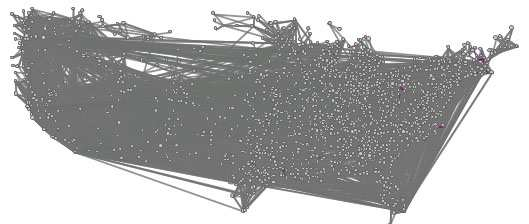
\includegraphics[width=100mm]{../figuras/cluttered-map.png}
  \caption[Trajetórias de voos nos Estados Unidos]{Trajetórias de voos nos Estados Unidos no período de uma semana. Fonte \citet{Zhou2013}.}
  \label{fig:exemplo-oclusao}
\end{figure}

  Para lidar com os problemas da oclusão, algumas técnicas têm sido
desenvolvidas por comunidades de visualização e da cartografia para a o estudo
de grandes conjuntos de dados de tráfego, como por exemplo, clusterização de
vértices\footcite{Schaeffer2007,Andrienko2011}, matrizes\footcite{Elmqvist2008}
e grides\footcite{JoWood2010}. Essas técnicas, no entanto, acabam usando
abstrações diferentes da representação baseada em linhas. Um outro tipo de
abstração pode ser obtido com uma técnica chamada \emph{bundling}, que tem sido
bastante utilizada na visualização massiva de dados do tráfego que utilizam a
representação de fluxos por linhas \citep{Zhou2013}. Algoritmos de
\emph{bundling} agrupam arestas similares e próximas, permitindo uma
representação única e compacta que reduz o número de arestas e a oclusão no
desenho. A Figura \ref{fig:exemplo-bund} ilustra a aplicação da técnica de
\emph{bundling}.  Quanto mais à esquerda, mais oclusão, e à direita, o
resultado final.

\begin{figure}[!htb]
  \centering
  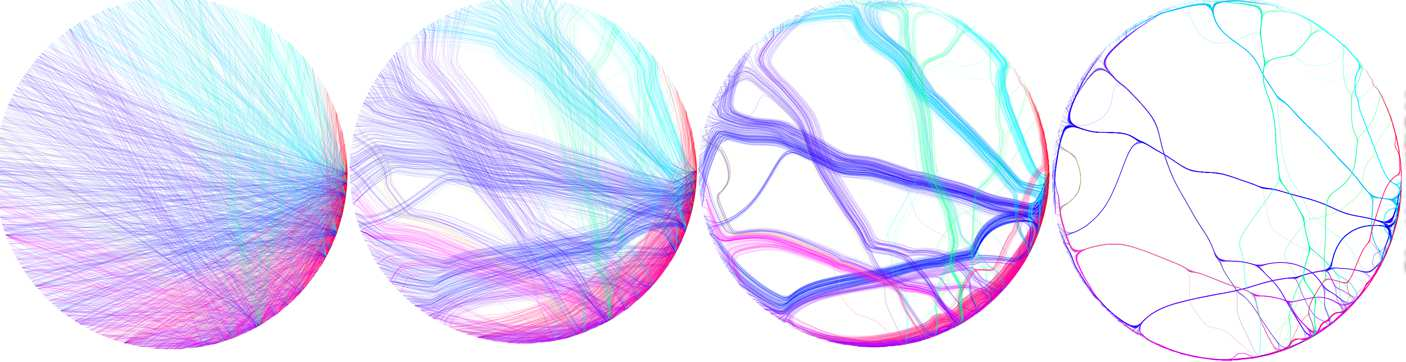
\includegraphics[width=1\textwidth]{../figuras/bundle-ex.png}
\caption[Exemplo de aplicação do \emph{bundling}]{Exemplo de aplicação do \emph{bundling}. Fonte: \citet{Hurter2012}.}
  \label{fig:exemplo-bund}
\end{figure}

  Uma variedade de métodos de \emph{bundling} têm sido apresentados por
pesquisadores, como métodos geométricos, hierárquicos e baseados em imagem
\citep{Lhuillier2017}. Recentemente, novos métodos viabilizaram a visualização
de grandes conjuntos de dados e em diferentes níveis de detalhes, como em
\citet{Klein2014}, que utilizam \emph{bundling} na visualização de milhares de
dados do tráfego aéreo. Eles mostram como a técnica destaca rotas comuns nos
voos e o grau de conexão entre diferentes aeroportos. O método utilizado
permite ainda uma abordagem multinível de acordo com parâmetros que
possibilitam o controle do \emph{bundling} em função da densidade de pontos no
espaço. Isso significa que é possível visualizar padrões globais entre grandes
áreas no mapa, que contemplem muitos pontos, e também padrões locais sobre
áreas menores com poucos pontos. Os autores também apresentam uma visualização
dinâmica para mostrar as mudanças no tráfego ao longo do tempo, agrupando os
voos em pequenos intervalos de tempo $\Delta t$ e aplicando o \emph{bundling}
nos dados de cada intervalo.

  Neste trabalho, focamos na visualização do fluxo de veículos no trânsito e as
relações de origem-destino (OD) que eles representam. Apresentamos uma
visualização dos dados utilizando \emph{bundling} para explorar os fluxos de
deslocamentos no trânsito da cidade e como eles impactam em vias com grandes
congestionamentos. Fazemos um novo estudo sobre visualização de dados do
tráfego projetando uma visualização para mostrar os fluxos em diferentes níveis
de detalhe. Utilizamos dados do tráfego de ônibus na cidade de São Paulo e
também dados gerados pelo InterSCSimulator, um simulador de cidades
inteligentes apresentado por \citet{mabs2017}.

\section{Objetivos e Contribuições}
  O objetivo desta pesquisa é explorar como o \emph{bundling} ajuda na
observação de padrões nos fluxos de deslocamento no tráfego de veículos de uma
grande cidade. Para isso, fazemos uma análise sobre as propriedades temporais e
espaciais dos dados do tráfego, sendo a direção e a densidade os principais
atributos que utilizaremos para responder a seguinte questão de pesquisa: \textbf{Como
o \emph{bundling} pode ser aplicado na análise de fluxos no trânsito da cidade
em diferentes níveis de detalhe?} 

 Para isso, apresentamos o InterSCityPlot, uma ferramenta livre e de código
aberto, para a análise de dados do tráfego de veículos que utiliza
\emph{bundling} para visualização dos dados do trânsito.  Exploramos o
\emph{bundling} em três aspectos: (1) abordagem multinível para visualizar
padrões globais (i.e. na escala da cidade), e locais (i.e. bairros, quadras e
ruas); (2) abordagem dinâmica para visualização de mudanças no padrão de fluxos
ao longo do tempo; (3) sua utilização com uma grande quantidade de dados do
trânsito em escala real de uma grande cidade, com mais de 4 milhões de
veículos.  Apresentamos também um conjunto de técnicas para mapear os atributos
dos dados com cores e texturas dentro de uma visualização sobre um mapa.

  Avaliaremos os resultados da visualização de maneira qualitativa e
quantitativa. Do ponto de vista qualitativo avaliaremos o que foi alcançado com
a visualização em comparação com outras visualizações, e também considerações
sobre suas vantagens e desvantagens. Além disso, posicionamos nossa proposta em
relação a outros trabalhos sobre visualização de dados de movimentação que
utilizam \emph{bundling}. Do ponto de vista quantitativo será avaliada a
escalabilidade da solução dado o tempo de processamento para gerar a
visualização de um certo conjunto de dados.

  Esperamos que a visualização a ser criada ajude na identificação das relações
entre as regiões da cidade que recebem maior fluxo, como esse fluxo se
distribui ao longo do tempo e como ele impacta em vias com grandes
congestionamentos. Desta forma, esta pesquisa potencialmente oferece as
seguintes contribuições científicas (CC) e contribuições técnicas (CT):

\begin{itemize}
  \item \textbf{CC} - avaliação do \emph{bundling} em multiníveis para análise de
padrões globais e locais do tráfego

  \item \textbf{CC} - avaliação da escalabilidade do \emph{bundling} na visualização de uma grande
quantidade de dados do tráfego de veículos

  \item \textbf{CC} - avaliação do \emph{bundling} dinâmico para análise de mudanças ao longo
do tempo

  \item \textbf{CT} - construção de uma ferramenta para visualização dos dados do tráfego
\end{itemize}

Esta pesquisa está sendo desenvolvida como parte do projeto InterSCity
\footnote{\rurl{interscity.org}} - INCT of the Future Internet for Smart
Cities. O objetivo do projeto é desenvolver pesquisas multidisciplinares em
infraestruturas de software para cidades inteligentes, produzindo contribuições
técnicas e científicas para a comunidade. Desta forma, o desenvolvimento desta
pesquisa de mestrado seguirá as diretrizes do projeto InterSCity para produzir
resultados que sejam reprodutíveis, bem como soluções de software
livre que possam ser mantidas adiante pela comunidade do projeto.
